%% bare_jrnl.tex
%% V1.4b
%% 2015/08/26
%% by Michael Shell
%% see http://www.michaelshell.org/
%% for current contact information.
%%
%% This is a skeleton file demonstrating the use of IEEEtran.cls
%% (requires IEEEtran.cls version 1.8b or later) with an IEEE
%% journal paper.
%%
%% Support sites:
%% http://www.michaelshell.org/tex/ieeetran/
%% http://www.ctan.org/pkg/ieeetran
%% and
%% http://www.ieee.org/


\documentclass[journal]{IEEEtran}

% *** GRAPHICS RELATED PACKAGES ***
%
\ifCLASSINFOpdf
   \usepackage[pdftex]{graphicx}
  % declare the path(s) where your graphic files are
   \graphicspath{{./vt-figures/}{../png/TIF/}}
  % and their extensions so you won't have to specify these with
  % every instance of \includegraphics
  \DeclareGraphicsExtensions{.tif,.jpeg,.png}
\else
  % or other class option (dvipsone, dvipdf, if not using dvips). graphicx
  % will default to the driver specified in the system graphics.cfg if no
  % driver is specified.
  % \usepackage[dvips]{graphicx}
  % declare the path(s) where your graphic files are
  % \graphicspath{{../eps/}}
  % and their extensions so you won't have to specify these with
  % every instance of \includegraphics
  % \DeclareGraphicsExtensions{.eps}
\fi

%
\usepackage{amsmath}
\usepackage{amsfonts}
\usepackage{float}
\usepackage{url}
% A popular package from the American Mathematical Society that provides
% many useful and powerful commands for dealing with mathematics.
%
% Note that the amsmath package sets \interdisplaylinepenalty to 10000
% thus preventing page breaks from occurring within multiline equations. Use:
\interdisplaylinepenalty=2500
% after loading amsmath to restore such page breaks as IEEEtran.cls normally
% does. amsmath.sty is already installed on most LaTeX systems. The latest
% version and documentation can be obtained at:
% http://www.ctan.org/pkg/amsmath





% correct bad hyphenation here
\hyphenation{op-tical net-works semi-conduc-tor}


\begin{document}
%
% paper title
% Titles are generally capitalized except for words such as a, an, and, as,
% at, but, by, for, in, nor, of, on, or, the, to and up, which are usually
% not capitalized unless they are the first or last word of the title.
% Linebreaks \\ can be used within to get better formatting as desired.
% Do not put math or special symbols in the title.
\title{\Huge Fun @ Constant Speed with Wolfram Alpha}
%
%
% author names and IEEE memberships
% note positions of commas and nonbreaking spaces ( ~ ) LaTeX will not break
% a structure at a ~ so this keeps an author's name from being broken across
% two lines.
% use \thanks{} to gain access to the first footnote area
% a separate \thanks must be used for each paragraph as LaTeX2e's \thanks
% was not built to handle multiple paragraphs
%

\author{{\it \LARGE Babak Makkinejad and Vadim Tugai}\IEEEmembership{}
% <-this % stops a space
% \thanks{M. Shell was with the Department
% of Electrical and Computer Engineering, Georgia Institute of Technology, Atlanta,
% GA, 30332 USA e-mail: (see http://www.michaelshell.org/contact.html).}% <-this % % stops a space
%\thanks{J. Doe and J. Doe are with Anonymous University.}% <-this % stops a space
%\thanks{Manuscript received April 19, 2005; revised August 26, 2015.}
}

% make the title area
\maketitle

% For peer review papers, you can put extra information on the cover
% page as needed:
% \ifCLASSOPTIONpeerreview
% \begin{center} \bfseries EDICS Category: 3-BBND \end{center}
% \fi
%
% For peerreview papers, this IEEEtran command inserts a page break and
% creates the second title. It will be ignored for other modes.
\IEEEpeerreviewmaketitle


\IEEEPARstart{T}{his note} is inspired by an earlier one$^1$ by Gerd Kortemeyer on the "Plug-and-chug" syndrome in physics education.  Here we extend the conventional approach of directly teaching elementary physics by formulas, which often would lead to the Plug-and-Chug phenomenon.  Starting from the old adage that "if you can't beat them, join them!", we propose that students engage in an open-ended exploration of physics by "plugging-and-chugging" various functions into formulas of physics theories.

Specifically, we are suggesting that students explore the ramifications for physics theories - without necessarily knowing how to derive the results of those theories themselves - in the case of the motion with constant speed in two dimensions.  In other words, what do physics theories tell us if we impose the constrain of uniform - but not rectilinear motion?  What do we learn?

We have relied extensively on the freely available symbolic computation and graphics capabilities of Wolfram Alpha$^2$.  We are not suggesting that Wolfram Alpha is the best such tool, only that it is free \& readily available and is already being used by many students. They use it for checking their homework formulas in calculus courses, for plotting 2-D and 3-D graphs - specially parametric functions - and to find roots of functions, as well as for matrix computations.  And it is not just physics and mathematics students that use it; economics majors use it to calculate such things as the Slutsky Substitution Effect and the Slutsky Income Effect.  In fact, Wolfram Alpha is very helpful for the more advanced levels of mathematics and related fields since it replaces TI-84 Graphics Calculator to carry out more complex calculations and programs.

The outline of this paper is as follows.  In section 1 we present the kinematic preliminaries of the uniform motion.  In section 2, we discuss possible physical situation that could give rise to such motion.  In section 3 we present the plots of a few trajectories for different choices of uniform motion.  Section 4 is devoted to the radiation emanating from a charged particle undergoing this motion.  Section 5 is a summary of what we have learned in our journey thus far.  Throughout, we include snap-shots of the Wolfram Alpha graphs with all the details so that our results could be duplicated by others.
\setcounter{secnumdepth}{1}
\section{\bf\large Modeling}
Let's consider two-dimensional motion of a particle with constant speed $b$, i.e. with constant magnitude of velocity $\vert\vec{v} \vert = b$. In Cartesian coordinates the most general form of this motion is given by:
\begin{equation}
\vec{v}(t)= b (\cos (\phi (t)), \sin (\phi (t)) ),
\label{eq:v-polar}
\end{equation}
where $\phi(t)$ is an arbitrary function of time. Geometrically, $\phi(t)$ is the angle between axis $x$ and velocity $\vec{v}$ measured in counter-clockwise direction (i.e. polar angle).
The acceleration of the particle can be obtained from (\ref{eq:v-polar}) by differentiation:

\begin{equation}
\vec{a}(t)= b \dot{\phi}(-\sin (\phi (t)), \cos (\phi (t)) ),
\label{eq:a-polar}
\end{equation}

and its magnitude is taking a very simple form $\vert \vec{a}(t) \vert = b\dot{\phi}(t)$.

\par We already know that given any two points A and B, a curve of any shape can connect the two points and that curve can always be traversed at constant speed.  Therefore the only defining feature of constant speed kinematics (other than speed is constant) is the connection between velocity and acceleration (how the curve is traversed), which must be perpendicular (assuming the velocity is smooth), so that to achieve such a motion the force must always be perpendicular to velocity. This is the defining feature of this problem which is demonstrated by the  orthogonality of equations 1 and 2.

The usual examples in introductory physics courses include a charged particle in a magnetic field, or an object that undergoes elastic collisions with an immovable object so that only direction changes (although for the latter the velocity would not be smooth and therefore the force needn't be perpendicular to the velocity).

An arbitrary function $g(t)= \dot{\phi}(t)$ can be selected to model movement of the particle. Physically, $\vec{a}$ from (\ref{eq:a-polar}) will represent classical (Newtonian) force (of an unspecified nature) acting on the particle. Calculating anti-derivative of $g(t)$ (i.e. indefinite integral $\int g(t) dt $) generates components of $\vec{v}$ in (\ref{eq:v-polar}). Alternatively, students can start from selecting an arbitrary function $\phi (t)$ and obtain $\vec{a(t)}$ by differentiation. In both cases anti-derivatives of $\vec{v}$'s components will represent position vector $\vec{r}(t)$ of the particle and can be used to plot its trajectory.

In a number of cases, students would be able to perform symbolic integration of velocity components in (\ref{eq:v-polar}) using Wolfram Alpha or similar tools. Frequently, however, obtaining them would require performing numerical integration, which (whilst giving them a feel of what mostly happens in real scientific/engineering life) would make students' projects "difficult rather than complex".

We noticed that symbolic integration features of Wolfram Alpha would not work effectively when functions $\phi(t)$ contain inverse trigonometric functions. In particular, they would, typically, fail to simplify the functions using expressions such as $\cos(\arcsin(t))=\pm\sqrt{1-t^2}$ before integrating them.  However, symbolic  integration can be used to analyze some of these cases by using an alternative representation for $\vec{v}(t)$:

\begin{equation}
\vec{v}(t)=b(f(t), {\pm\sqrt{1-f^2(t)}} \ ),
\label{eq:v-frep}
\end{equation}

where $f(t)$ is also an arbitrary function of time.  Note that this function is related to the function $\phi (t)$ via 

\begin{equation}
f (t) = \cos (\phi (t))
\label{eq:f-from-phi}
\end{equation}

\par The $\pm$ symbol in the expression (\ref{eq:v-frep}) highlights that (real) function $f(t)$ by itself cannot model changes of sign of velocity components (which $\phi(t)$, certainly can). Discussing this "lost sign information" with the students can lead naturally to emphasizing the importance of keeping track on functions' domain and co-domain areas to avoid "plug and chug" pitfalls.

\par As will be shown in the next section, defining these functions in a piece-wise manner in lieu of using the $\pm$ symbol illustrates the significance of constants of integration in order for the calculated expressions for velocities and trajectories to be "physical" . Simply ignoring the constants of integration (i.e. setting them to 0) represents another type of case where "plug and chug" approach can easily lead to incorrect results.  Furthermore, not all choices of of $g(t)$ (or $\phi (t)$) and initial conditions $\phi (t_0)$ would be physically meaningful since they lead to complex-valued functions for the components of velocity or position vectors.

\section{\bf\large Trajectories and Accelerations}
\par Let's first consider the simplest case of constant-magnitude acceleration $g(t)= const = \omega$. We start from integrating $g(t)$, which yields $\phi(t)= b \omega t + C_v$. We then substitute $\phi (t)$ into (\ref{eq:v-polar}) and integrate again to obtain:

\begin{equation}
\vec{r}(t)= {b\over \omega} \left( \sin (\omega t + C_v) + \omega C_x, -\cos (\omega t + C_v) + \omega C_y \right)
\label{eq:uniform-traject}
\end{equation}

These expressions represent uniform circular motion with radius $b/\omega$ and angular frequency $\omega$.  Changes to constant $C_v$ (first integration) do not influence the shape of the trajectory (nor its size) as they correspond to "time shifts" (by $C_v / \omega$). Constants $C_x$ and $C_y$ (second integration) do not change trajectory's shape/size plot either, as they only influence its position on the coordinate plane.

Let's now analyze the modeling function $g(t)=exp(kt)$. The expression for $\phi(t)$ becomes: $\phi(t)= 1/k \exp(k t)+C_v$ and for $\vec{v}$ and $\vec{r}$ we obtain:

\begin{equation}
\begin{aligned}
&\vec{v}(t)= b \left( \cos (\frac{e^{kt}}{k}  + C_v ), \sin (\frac{e^{kt}}{k} + C_v  ) \right),\\
&r_x(t)= \frac{b}{k} \left( \cos(C_v) Ci (\frac{e^{kt}}{k}  + C_v ) - \sin (C_v) Si (\frac{e^{kt}}{k}  + C_v ) \right), \\
&r_y(t)= \frac{b}{k} \left( \sin(C_v) Ci (\frac{e^{kt}}{k}  + C_v ) - \cos (C_v) Si (\frac{e^{kt}}{k}  + C_v ))\right)
\end{aligned}
\label{eq:expon-traject}
\end{equation}

where $Si$ and $Ci$ are sine and cosine integrals$^4$, and where constants of integration $C_x$ and $C_y$ are set to $0$. The trajectory is plotted below.
\begin{figure}[H]
\includegraphics[width=7.5cm]{FIG1_1}
\caption{\ Plot of trajectory described by equation (\ref{eq:expon-traject}), with $b=k=1, C_v={\pi\over 2} -1$ and $ -4 \leq t \leq 4 $ \bigskip}
\centering
\label{fig:phiexp-traj}
\end{figure} 
We noticed that choosing elementary functions for $\phi(t)$ often lead to spiral trajectories.

It is instructive to model uniform circular motion as well as simple-looking "deviations" from such motion by using $f(t)$ representation from (\ref{eq:v-frep}). For example, students can be asked to analyze the case $f(t)= k \sin (t) $ i.e.: 

\begin{equation}
f(t)= k \sin (t) \text{, where } 0 < k \leq 1
\label{eq:sintk-repr}
\end{equation}

We will not be analyzing cases $k>1$ as they lead to imaginary values for $v_y$. As mentioned in the first section, attempts to directly analyze cases of $k\ne 1$ in $\phi$-representation given by:

\begin{equation}
\phi(t)= \arccos \left( { k \sin (t) } \right)
\label{eq:sintk-phi-repr}
\end{equation}
(cf. (\ref{eq:f-from-phi})) also lead to complications when $k\ne 1$ as Wolfram Alpha cannot numerically integrate the corresponding function for $v_y$.

It is rather natural for the students to simply ignore the $\pm$ sign in (\ref{eq:sintk-repr}) and obtain the following expressions for vectors of velocity and position:
%
\begin{equation}
\begin{aligned}
&\vec{v}(t)=b\left( k \sin(t), {\sqrt{1-k\sin ^2(t)}} \right )
\\
&\vec{r}(t) = b \left( -{k \cos(t)}+C_x, E(t|k)+C_y \right),
\end{aligned}
\label{eq:sintk-vr-naive}
\end{equation}

where $E(t|k)$ denotes Elliptical integral of the second kind. Differentiation of (\ref{eq:sintk-repr}) gives corresponding acceleration:
\begin{equation}
\vec{a}(t) = bk \left( { \cos(t)}, - { {\sin t \cos t } \over  \sqrt{1 - k \sin ^2 t}} \right)
\label{eq:sintk-a}
\end{equation}


\par Let's start our analysis from the uniform circular motion, i.e. from the case $k=1$. In effect, we are using $r_y=\sqrt{cos^2(t)}\tan (t)$ instead of an Elliptic function, which does not change the plot below. The corresponding trajectory and accelerations are plotted below.

\begin{figure}[H]
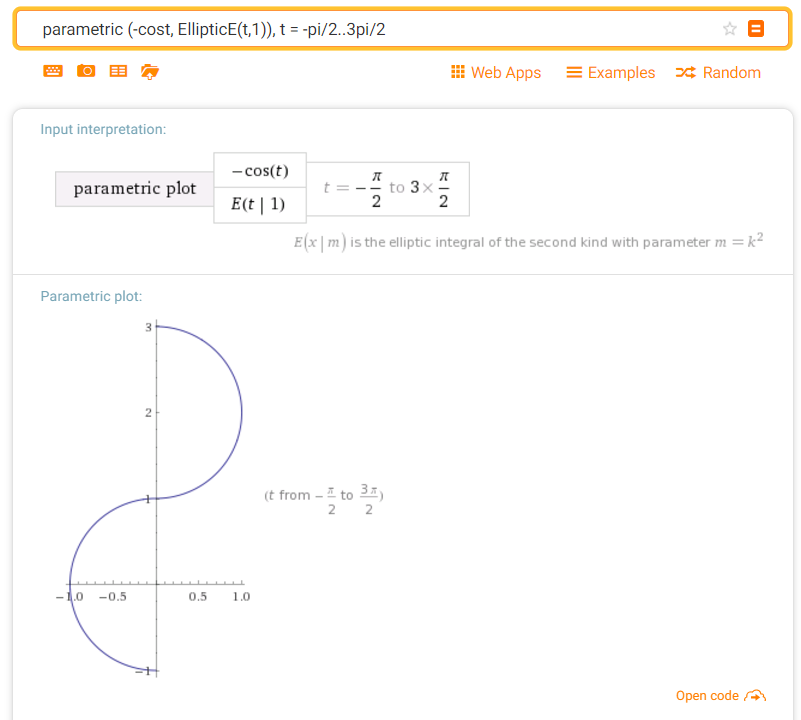
\includegraphics[width=7.5cm]{sintk-traj-uniform-naive}
\caption{\ Plot of the motion described by equation (\ref{eq:sintk-vr-naive}), with $b=1$, $k=1$, $C_v=0$ and $ - { \pi \over 2 }  \leq t \leq { 3 \over 2 } \pi $ \bigskip}
\centering
\label{fig:sintk-traj-uniform-naive}
\end{figure}

\begin{figure}[H]
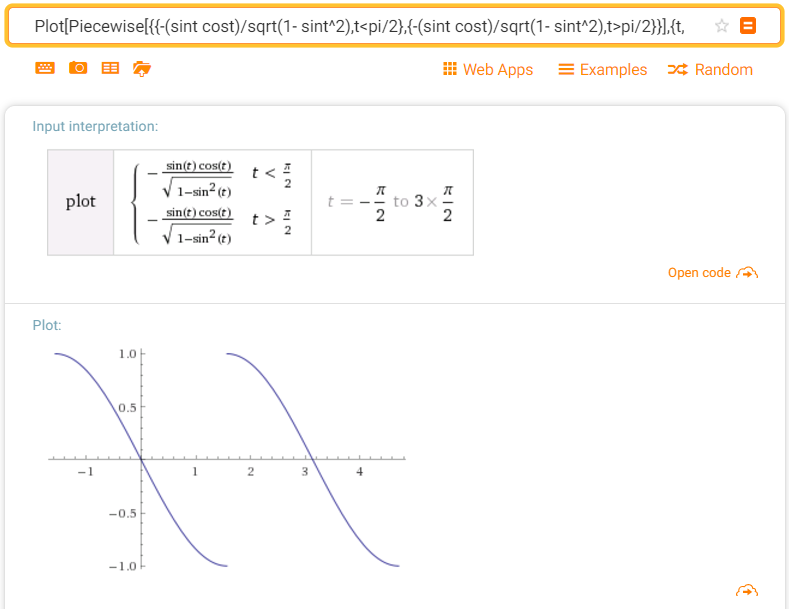
\includegraphics[width=7.5cm]{sintk-accel-uniform-naive}
\caption{\ Plot of acceleration component $a_y$ described by equation (\ref{eq:sintk-a}), with $b=1$, $k=1$ and $ - { \pi \over 2 }  \leq t \leq { 3 \over 2 } \pi $ \bigskip}
\centering
\label{fig:sintk-accel-uniform-naive}
\end{figure}


There is an obvious problem with these results: the trajectory is no longer circular. Furthermore, $v_y$ is no longer smooth and, as a result, $a_y$ becomes discontinuous at $t={\pi \over 2} + n\pi$  (where $n \in \mathbb {Z}$). These issues are due to the "loss of sign information" for $v_y$ component. They demonstrate that we, generally, cannot ignore the $\pm$ sign in (\ref{eq:v-frep}). Instead, this "lost" sign needs to be reintroduced as a function of time. 

In the case $k=1$ the sign can be reintroduced easily since we know what that it should behave as sign of $\cos(t)$ for uniform circular motion. Let's try to apply the same "sign recovery" approach for cases $k < 1$ and see where it leads us.  Our first attempt is:

\begin{equation}
v_y(t)=
\begin{cases} 
b \sqrt{1-k\sin^2(t)} & \text{if } -{\pi \over 2} + n\pi < t < {\pi \over 2} + n\pi \\
- b \sqrt{1-k\sin^2(t)} & \text{if } {\pi \over 2} + n\pi < t < {3\pi \over 2} + n\pi
\end{cases}
\label{eq:sintk-vy-pieces1}
\end{equation}

(where $n \in \mathbb {Z}$), does not produce satisfactory results as $v_y$ would become discontinuous when $k<1$. To address the issue we need to "stitch" the pieces by adding or subtracting $b\sqrt{1-k}$: 

\begin{equation}
v_y(t)=
\begin{cases} 
b \sqrt{1-k\sin^2(t)} - b\sqrt{1-k} & \text{if } -{\pi \over 2} < t < {\pi \over 2} \\
- b \sqrt{1-k\sin^2(t)} + b\sqrt{1-k}& \text{if } {\pi \over 2} < t < {3\pi \over 2} 
\end{cases}
\label{eq:sintk-vy-pieces2}
\end{equation}

(hereafter we will be omitting the $+n\pi$ terms shown in (\ref{eq:sintk-vy-pieces1}))

Piece-wise integration of (\ref{eq:sintk-vy-pieces2}) yields:

\begin{equation}
r_y(t)=
\begin{cases} 
b E(t|k)-b\sqrt{1-k}t+C_y & \text{if } -{\pi \over 2} < t < {\pi \over 2} \\
- b E(t|k)+b\sqrt{1-k}t+C'_y & \text{if } {\pi \over 2} < t < {3\pi \over 2} 
\end{cases}\\
\label{eq:sintk-ry-pieces}
\end{equation}

It should be noted that the constants of integration $C_y$ and $C'_y$ are not independent. In particular, if students attempt to set constant of integration for both pieces (independently) to $0$ the trajectory would fail to remain circular for $k=1$. This issue demonstrates importance of analyzing constants of integration even when the task does not have  particular initial conditions specified. To "stitch" the pieces of trajectory we need to set:

\begin{equation}
C'_y =C_y+2bE({\pi \over 2}|k)-b\sqrt{1-k}\pi 
\label{eq:sintk-ry-coi}
\end{equation}

The corresponding trajectory is plotted below.

\begin{figure}[H]
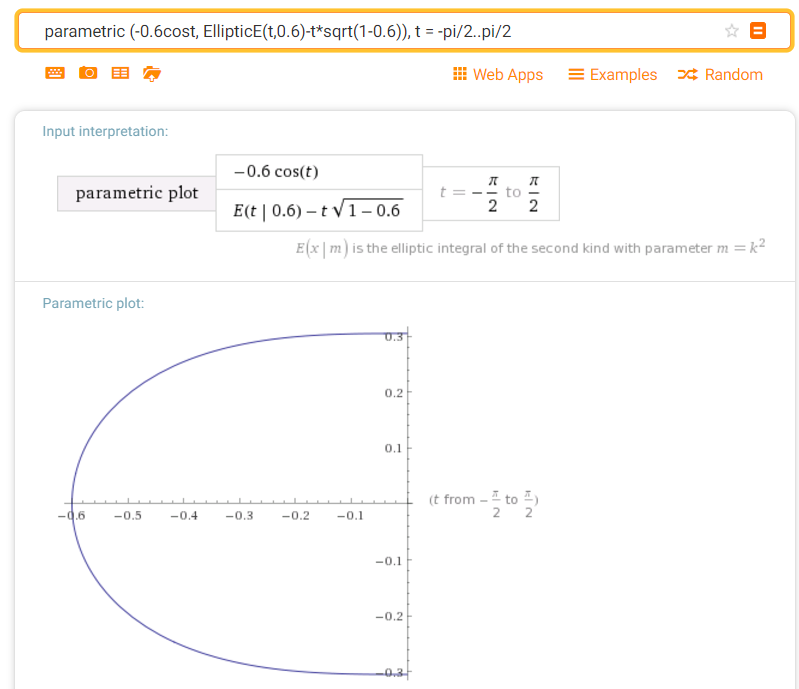
\includegraphics[width=7.5cm]{r_y-sintk-b-piece1}
\caption{\ Plot of trajectory described by equations (\ref{eq:sintk-ry-pieces}) and (\ref{eq:sintk-ry-coi}), with $b=1$, $k=0.6$ and $ - { \pi \over 2 }  \leq t \leq { 3 \over 2 } \pi $ \bigskip}
\centering
\label{fig:r_y-sintk-b}
\end{figure}

and

\begin{figure}[H]
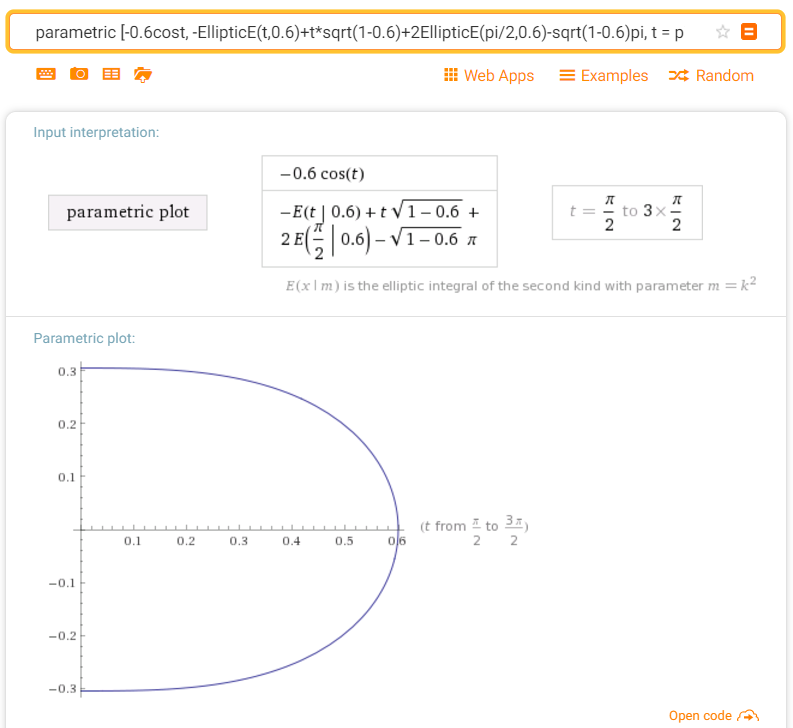
\includegraphics[width=7.5cm]{r_y-sintk-b-piece2}
\caption{\ Plot of trajectory described by equations (\ref{eq:sintk-ry-pieces}) and (\ref{eq:sintk-ry-coi}), with $b=1$, $k=0.6$ and $ - { \pi \over 2 }  \leq t \leq { 3 \over 2 } \pi $ \bigskip}
\centering
\label{fig:r_y-sintk-b}
\end{figure}

As a bonus problem students can be asked to demonstrate graphically that this curve is not an ellipse.

It would appear at this stage, that the expression (\ref{eq:sintk-vy-pieces2}) represents physically meaningful behavior of a particle. Analysis of accelerations, however, reveals other issues. Differentiation of (\ref{eq:sintk-vy-pieces2}) yields:

\begin{equation}
a_y(t)=
\begin{cases} 
- bk { {\sin t \cos t } \over  \sqrt{1 - k \sin ^2 t}} 
& \text{if } -{\pi \over 2} < t < {\pi \over 2} \\
bk { {\sin t \cos t } \over  \sqrt{1 - k \sin ^2 t}}
& \text{if } {\pi \over 2} < t < {3\pi \over 2} ,
\end{cases}
\label{eq:sintk-a-pieces}
\end{equation}

and in the case of $k=1$ (and $b=1$) we obtain a regular graph of $-\sin(t)$. Cases $k<1$, however, give significantly different results and the function $a_y(t)$ is no longer smooth (regardless of how close we are to $k=1$!):
%
\begin{figure}[H]
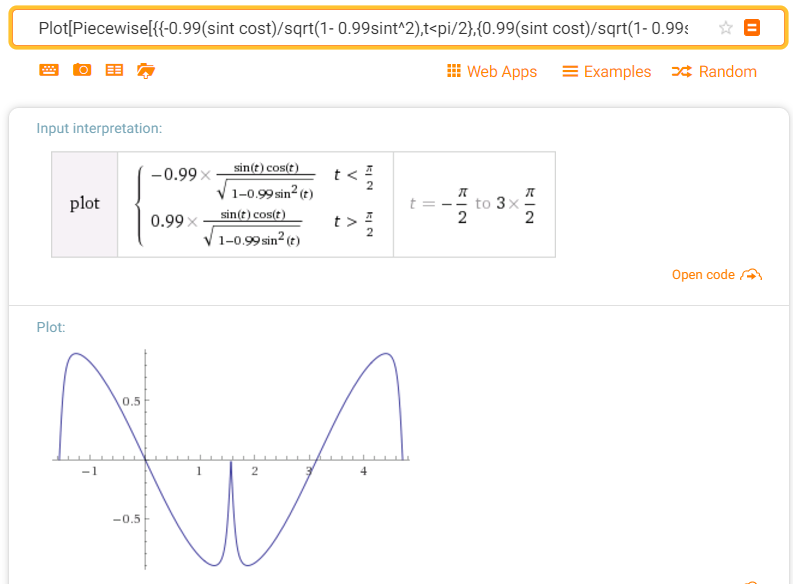
\includegraphics[width=7.5cm]{sintk-accel-pieces}
\caption{\ Plot of acceleration component $a_y$ described by equation (\ref{eq:sintk-a-pieces}), with $b=1$, $k=0.99$ and $ - { \pi \over 2 }  \leq t \leq { 3 \over 2 } \pi $ \bigskip}
\centering
\label{fig:sintk-accel-pieces}
\end{figure}


If we compare this outcome with the behavior of $a_y(t)$ for $k<1$ in the "apparently naive" representation (\ref{eq:sintk-a}), we will find that in the later case the function is smooth:

\begin{figure}[H]
% TBA
\caption{\ Graph of acceleration component $a_y$ described by equation (\ref{eq:sintk-a}), with $b=1$, $k=0.99$ and $ - { \pi \over 2 }  \leq t \leq { 3 \over 2 } \pi $ \bigskip}
\centering
\label{fig:sintk-accel-naive}
\end{figure}

It is also interesting to compare the plots of $\vec{a}(t)$ in these two cases. It turns out, the plots look identical (for the same value of $k$). However, in the "apparently naive" case the point on this plot representing the acceleration of the moving particle draws "figure eight" (as time passes), whilst the piece wise representation (\ref{eq:sintk-a-pieces}) corresponds to point moving non-smoothly as arrows on the plot below illustrate:

\begin{figure}[H]
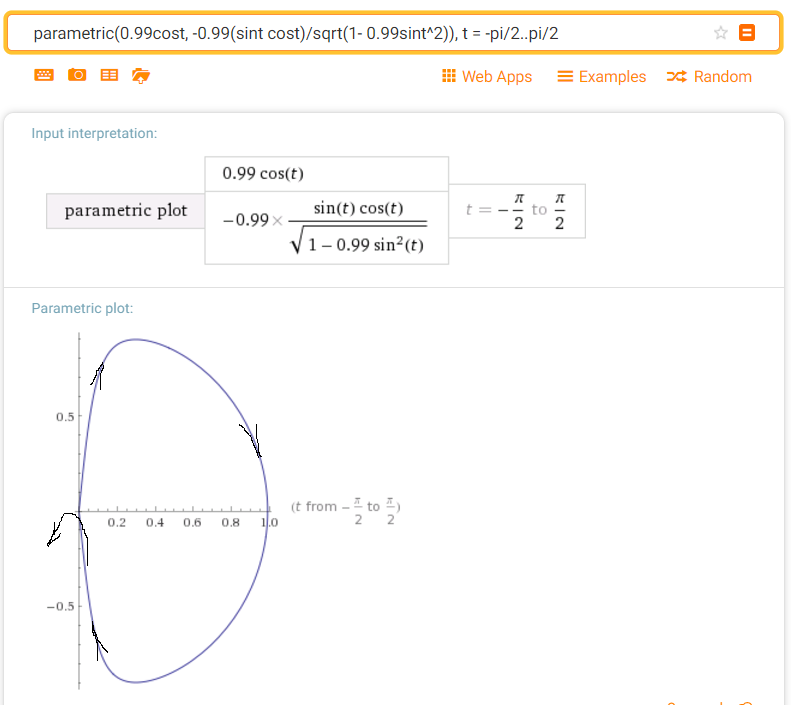
\includegraphics[width=7.5cm]{sintk-accel-plot-piece1}
\caption{\ Plot of acceleration $\vec{a}$ described by equation (\ref{eq:sintk-a-pieces}), with $b=1$, $k=0.99$ and $ - { \pi \over 2 }  \leq t \leq { 3 \over 2 } \pi $ \bigskip}
\centering
\label{fig:sintk-accel-plot-pieces}
\end{figure}

and

\begin{figure}[H]
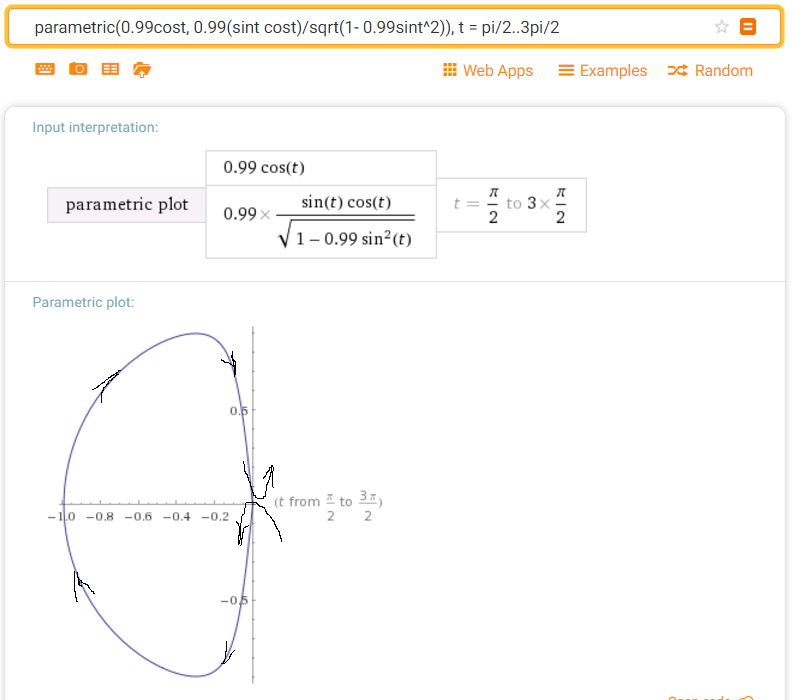
\includegraphics[width=7.5cm]{sintk-accel-plot-piece2}
\caption{\ Plot of acceleration $\vec{a}$ described by equation (\ref{eq:sintk-a-pieces}), with $b=1$, $k=0.99$ and $ - { \pi \over 2 }  \leq t \leq { 3 \over 2 } \pi $ \bigskip}
\centering
\label{fig:sintk-accel-plot-pieces}
\end{figure}

Analysis of trajectories for cases $k<1$ in "apparently naive" representation shows that they are not affected by the smoothness-of-$v_y$ (continuity of $r_y$) issues discussed above for the case $k=1$, even though from (\ref{eq:sintk-vr-naive}) we obtain $k<1$ trajectories that are no longer closed and very similar to the one shown on Fig \ref{fig:sintk-traj-uniform-naive} above:

\begin{figure}[H]
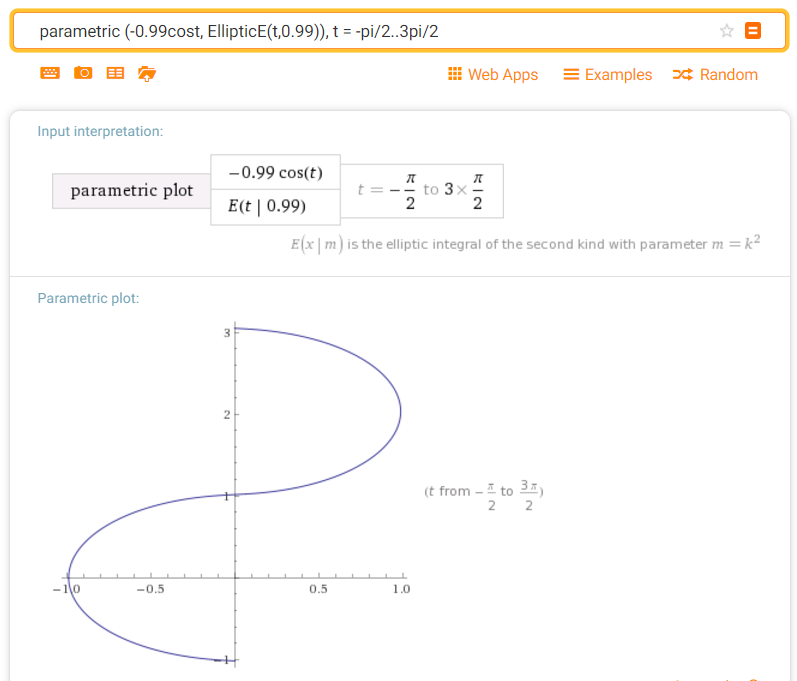
\includegraphics[width=7.5cm]{traject-sintk-naive}
\caption{\ Plot of trajectory described by equation (\ref{eq:sintk-vr-naive}), with $b=1$, $k=0.99$ \bigskip}
\centering
\label{fig:traject-sintk-naive}
\end{figure}


Thus, lack of smoothness of $a_y$ in (\ref{eq:sintk-a-pieces}) (see Fig \ref{fig:sintk-accel-pieces}) appears to be the "price to pay" for demanding that magnitude of velocity to remain constant whilst trajectory remain a close curve (deformation of a circle).

On the other hand, letting $b=1$ and $g(f,t)=kf^2(t)$, we obtain $ f(t) = \sqrt{1+{k^2}{t^2}}^{\ -1}$, which, upon integration, gives the displacement vector:

\begin{align}
\vec{r}(t)=({ArcSinh(kt)\over k}, {tArcSinh(kt)} \ ),
\end{align} with the trajectory:

\begin{figure}[H]
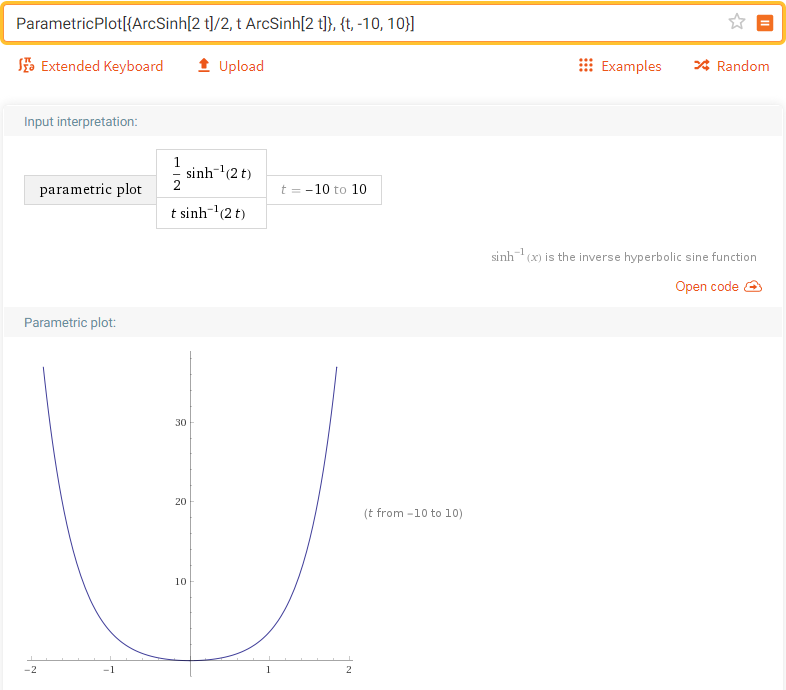
\includegraphics[width=6.75cm]{fig11}
\caption{\ Plot of trajectory described by equation (16), $k=2, -10. \leq t \leq 9. $\bigskip}
\centering
\end{figure}

For comparison purposes, we note here that the parametric equation of an ellipse, with semi-major axis a and b, is given by 
$\rho = \pm \sqrt(a^2cos^2t+ b^2sin^2t) $, and 
$\phi = Arctan[b/aTan(t)]$ in polar coordinates.


Many more such examples many be constructed, limited only by one's inventiveness.  And all of them would be exhibiting constant speed in two dimensions regardless of the specific form that their trajectory takes.  Students could try different functions and construct the trajectory of the motion.  Depending on the choice of the function $g(f,t)$ one might be able to determine the acceleration using a table of integrals$^2$.  The absence of a closed-form for the integrals serves the important purpose of showing that not all problem have neat, closed-form solutions and how quickly one can find oneself in such situations.  

\par For example, things also become quite interesting when one intentionally deviates from from uniform circular motion by replacing $b$ with something slightly different than $1$, say $1.01$ and by letting $f(t)= sin(t)$ (this corresponds to letting $\omega = 1$, without loss of generality):

\begin{align}
\vec{v}(t)=(sin(t), {\sqrt{1.01-sin^2(t)}\ )},
\end{align}

the trajectory of the motion becomes:

\begin{figure}[H]
\includegraphics[width=6.75cm]{FIG12.PNG}
\caption{\ Plot of trajectory described by equation (17), $ -10. \leq t \leq 10. $.\bigskip}
\centering
\end{figure} 

In order to verify that such motions are indeed physical, let's start from the corresponding map of forces, i.e. with the plot for acceleration corresponding to (11). 
\begin{figure}[H]
\includegraphics[width=6.75cm]{FIG13.PNG}
\caption{\ Plot of acceleration for motion described by equation (17), $ \pi/2 \leq t \leq \pi. $.\bigskip}
\centering
\end{figure}

The piece-wise plot for acceleration is continuous and smooth and by integrating the $x$ and $y$ components of the acceleration we would arrive at the expression similar to (12), except there will be constants of integration. The point is that to arrive at the physical answers for $V_x$ and $V_y$ we need to select these constants of integration based on the initial conditions, considered separately for each piece (in other words, based on performing "stitching" for plot of velocity). 

%comment out in the interest of brevioty
%A more complicated case, when $f(t)$ is set to the Legendre Polynomial$^3$ of %order $2$:

%\begin{align}
%\vec{v}(t)=({0.5}(1+3cos^2(t)), \sqrt{2.0 - {0.25}(1 + 3cos^2(t))^2},
%\end{align}

%gives the trajectory:

%\begin{figure}[H]
%\includegraphics[width=6.75cm]{FIG3.PNG}
%\caption{\ Plot of trajectory described by equation (18), $ -10. \leq t \leq %10. $ t.\bigskip}
%\centering
%\end{figure}


\section{\bf\large The Electromagnetic Field}

Most of interactions at macroscopic level are caused by central forces, which (in general) influence both direction and magnitude of the particle's velocity. There is only one notable exception --- Lorentz force for a charged particle moving in a magnetic field. Acceleration of the particle is described by the following equation:
\begin{align}
m \vec{a}(t)= q \vec{v}(t) \times \vec{B}(t),
\end{align}
where $m$ is mass of the particle, $q$ its electric charge and $\vec{B}(t)$ is magnetic field (aka magnetic flux density). The vector product operation in this formula causes the acceleration to always be normal to the velocity vector, thus not allowing its magnitude (i.e. particle's speed) to be affected.

Equations for a particle moving in plane $xy$ (i.e. two-dimensional movements) can be easily rewritten in component form:
\begin{align}
\vec{a}(t)= \frac{q}{m} B_z(t)( v_y(t), - v_x(t)), 
\end{align}
where $B_z(t)$ is projection of $\vec{B}(t)$ onto z-axis (forming right-handed coordinate system with the coordinate axis $x$ and $y$). Taking (1) into account we obtain:
\begin{align}
\vec{a}(t)= \frac{1}{m} q b \vec{B}_z(t) ( \sin \phi (t), - \cos (t) ), 
\end{align}
which allows us to determine the physical interpretation for the function $g(t)$ introduced above: 
\begin{align}
g(t)= - \frac{q}{m} B_z(t).
\end{align}
In other words, $g(t)$ defines time how external magnetic force (acting within the plane) changes with time.

\par As a bonus problem, students could be asked to analyze, using similar methods, but with (2-dimensional) reference frame moving with the particle. In general, any central forces would produce only trivial solutions (such as uniform circular motion). The only non-trivial physical context for motion with constant speed is a charged particle moving (without friction) in a variable magnetic field.  Physically, that would correspond to either a "rock" (when tangential component of $\vec{v}$ is always constant) or a "rocket" (when tangential component of $\vec{v}$ is changing as a function of time) under the influence of forces that remain always perpendicular to the speed.  An example of such forces would be the Lorenz forces from multiple and/or variable sources of magnetic fields.  Of course, in that case, our rock/rocket would need to be electrically charged!


\section{\bf\large Radiated Power}
The Larmor formula for the total power radiated by a non-relativistic point charge under acceleration is given by$^5$:
\begin{align}
P={2 \over 3}{\frac {q^{2}a^{2}}{4\pi \varepsilon _{0}c^{3}}}={\frac {q^{2}a^{2}}{6\pi \varepsilon _{0}c^{3}}}{\mbox{ (SI units)}} ,
\end{align}
and by 
\begin{align}
P={\frac {2q^{2}\gamma ^{6}}{3c}}\left[({\dot {\boldsymbol {\beta }}})^{2}-({\boldsymbol {\beta }}\times {\dot {\boldsymbol {\beta }}})^{2}\right] ,
\end{align}
in the relativistic case.  Both equations could have singularity for certain choices of parameters and functions describing the uniform motion.  Different choices lead to different pattern of radiated power.  

Below, we have plotted such an example below - in units of ${\frac {q^{2}}{6\pi \varepsilon _{0}c^{3}}}$ - for the motion corresponding to eq. (17).
\begin{figure}[H]
\includegraphics[width=6.75cm]{FIG14.PNG}
\caption{\ Plot of the radiated Power described by equation (17), $ -5. \leq t \leq 5. $\bigskip}
\centering
\end{figure}
%
%and 
%\begin{figure}[H]
%\includegraphics[width=6.75cm]{FIG6.PNG}
%\caption{\ Plot of the radiated Power described by equation (18), $ -5. \leq t %\leq 5. $\bigskip}
%\centering
%\end{figure}
%
Any motion that has uniform speed but not constant velocity and electric charge could be made to radiate infinite power.  Of course this is not true in practice but very large amounts of power could be made to radiate from such a charge.  And that energy must come from somewhere.  One could discuss this briefly. 

\section{\bf\large Summary}
\par This paper has been mainly about two specific parameterizations of constant speed trajectories, equations 1 and 3, and how one has to be careful with each choice of parameterization (the former has trickiness with trig functions, the latter has trickiness with signs). The two parameterizations are the most natural one but we observe here that they are not the only ones: indeed, if one parameterizes the curve by arclength rather than time (which is a common thing to do in differential geometry), then one automatically has a constant speed curve.

\par Furthermore, we have demonstrated the utility of using the online tool - Wolfram Alpha - in exploring the ramifications of this constant speed trajectories for various choices of functions; using its numerical and graphical capabilities.

\par We believe that some or all of these material, which is at a "higher level" of "Plug-and-chug" could encourage students in exploring and developing deeper understandings in the study of physics and mathematics.  
\par There are multiple directions that one could take the students from here.  For example, it could be interesting to discuss with then how a single scalar constraint on velocity vector $\vert\vec{v}\vert=b$ reduces degrees of freedom for acceleration $\vec{a(t)}$ so it becomes fully represented by a scalar function $g(t)$; which is due to considering 2-dimensional motions only.


\begin{thebibliography}{99}

\bibitem{article} Gerd Kortemeyer, "The Losing Battle against Plug-and-Chug", {\it Phys. Teach.\/}, 54, 14 (2016).

\bibitem{url1} Wolfram Alpha, {\url{https://www.wolframalpha.com/}}
Online; accessed August 28, 2019.

\bibitem{article} Marcos D. Caballero, "Integrating Numerical Computation into the Modeling Instruction Curriculum", {\it Phys. Teach.\/}, 52, 38 (2014).

\bibitem{book1} David Zwillinger {\it Table of Integrals, Series, and Products \/} 8th. edition (Academic Press, New York, 2014).

\bibitem{book2} M. Abromovitz, and I. A. Stegun,  {\it Handbook of Mathematical Functions \/}, (Dover Publications, New York, 1965). Also accessible from {\url{http://dlmf.nist.gov}}

\bibitem{url2} Wikipedia, {\url{https://en.wikipedia.org/wiki/Larmor_formula/}} Online; last accessed February 28, 2017.

\end{thebibliography}

% biography section
% 
% If you have an EPS/PDF photo (graphicx package needed) extra braces are
% needed around the contents of the optional argument to biography to prevent
% the LaTeX parser from getting confused when it sees the complicated
% \includegraphics command within an optional argument. (You could create
% your own custom macro containing the \includegraphics command to make things
% simpler here.)
%\begin{IEEEbiography}[{\includegraphics[width=1in,height=1.25in,clip,keepaspectratio]{mshell}}]{Michael Shell}
% or if you just want to reserve a space for a photo:

%\begin{IEEEbiography}{Babak Makkinejad}
%Babak Makkinejad is a senior software developer at General Motors and holds a Ph.D. in %Physics from the University of Michigan in Ann Arbor.
%\end{IEEEbiography}

% if you will not have a photo at all:
\begin{IEEEbiographynophoto}{Babak Makkinejad}
is a senior software developer with General Motors and holds a Ph.D. in Physics from the University of Michigan in Ann Arbor, USA.
\end{IEEEbiographynophoto}
\begin{IEEEbiographynophoto}{Vadim Tugai}
is a consultant with AT{\&}T and holds a Ph.D. in Physics and Mathematics from Kharkov Mono-crystal Institute, Ukraine.
\end{IEEEbiographynophoto}

% insert where needed to balance the two columns on the last page with
% biographies
%\newpage

%\begin{IEEEbiographynophoto}{Babak Makkinejad}
%Babak Makkinejad is a consultant at HP Enterprise and holds a Ph.D. in %Physics from the University of Michigan in Ann Arbor.
%\end{IEEEbiographynophoto}

% You can push biographies down or up by placing
% a \vfill before or after them. The appropriate
% use of \vfill depends on what kind of text is
% on the last page and whether or not the columns
% are being equalized.

%\vfill

% Can be used to pull up biographies so that the bottom of the last one
% is flush with the other column.
%\enlargethispage{-5in}



% that's all folks
\end{document}


